% !TeX program = xelatex
% Release builds use XeLaTeX or Tectonic's XeTeX engine; pdfLaTeX is not the
% supported source-bundle target.
\documentclass[11pt]{article}

\usepackage[T1]{fontenc}
\usepackage[utf8]{inputenc}
\usepackage[margin=1in]{geometry}
\usepackage{microtype}
\usepackage{amsmath,amssymb}
\usepackage{booktabs}
\usepackage{array}
\usepackage{tabularx}
\usepackage{longtable}
\usepackage{enumitem}
\usepackage{graphicx}
\usepackage{xcolor}
\usepackage{hyperref}
\usepackage{caption}
\usepackage{subcaption}
\usepackage{float}

\newcommand{\PaperTableStretch}{1.22}
\renewcommand{\arraystretch}{\PaperTableStretch}
\newcommand{\PaperStack}[2]{\shortstack[l]{#1\\#2}}
\newcommand{\PaperStackHead}[2]{\shortstack[c]{#1\\#2}}
\newcolumntype{Y}{>{\raggedright\arraybackslash}X}
\newif\ifshowclaimmanifest
\showclaimmanifesttrue

\definecolor{accentBlue}{HTML}{1D3557}
\definecolor{accentGold}{HTML}{B08900}

\hypersetup{
  colorlinks=true,
  linkcolor=accentBlue,
  citecolor=accentBlue,
  urlcolor=accentBlue
}

\IfFileExists{generated/tex/build_meta.tex}{\newcommand{\PrimaryRepoSHA}{07856f2-dirty}
\newcommand{\PrimaryRepoCommitDate}{2026-04-26}
\newcommand{\UpstreamRepoSHA}{72ce36b-dirty}
\newcommand{\UpstreamRepoCommitDate}{2026-04-26}
\newcommand{\SamRepoSHA}{47acc8d-dirty}
\newcommand{\SamRepoCommitDate}{2026-04-23}
}{
  \newcommand{\PrimaryRepoSHA}{metadata unavailable}
  \newcommand{\PrimaryRepoFullSHA}{metadata unavailable}
  \newcommand{\PrimaryRepoCommitDate}{metadata unavailable}
  \newcommand{\UpstreamRepoSHA}{not used}
  \newcommand{\UpstreamRepoCommitDate}{not used}
  \newcommand{\ScaleoutRepoSHA}{pending artifact bundle}
  \newcommand{\ScaleoutRepoCommitDate}{pending artifact bundle}
}
\newcommand{\DraftDate}{\PrimaryRepoCommitDate}

\title{VLMaxxing through FrameMogging\thanks{Look, they said attention was all you needed, well we got your attention with this title.}\\Training-Free Anti-Recomputation for Video Vision-Language Models}
\author{
  JF Bastien\\
  \texttt{paper@jfbastien.com}
  \and
  Sam D'Amico\\
  \texttt{sam@impulselabs.com}
}
\date{\DraftDate}

\begin{document}
\maketitle

\begin{abstract}
Video VLMs keep paying to understand pixels they have already understood, and
component-level efficiency wins are easy to misread as end-to-end wall-clock
wins unless the accelerated stage's share is reported. We study this
training-free anti-recomputation problem across three non-interchangeable
regimes: first-pass vision pruning on fresh videos, after-ingest follow-up
queries on the same video, and streaming/deployment reuse. First, we derive
\emph{C-CEILING}: stage-local speedups only survive in proportion to the
wall-clock share the accelerated stage actually owns. The ceiling explains why
the pooled n=60 composition attempt is a null rather than a multiplier. Second,
we measure \emph{C-VISION}: on Gemma 4-E4B-4bit, vision-tower pruning gives
1.113$\times$ to 1.407$\times$ first-pass gains across clean and advisory
holdout cells, and a matched Qwen cross-architecture probe lands at
1.044$\times$ observed versus 1.043$\times$ predicted. Third, we characterize
\emph{C-PERSIST}: unrepaired Qwen2.5-VL-7B same-video follow-ups drop to
815\,ms median at 47.2$\times$ speedup at 8 frames and 807\,ms at
91.1$\times$ at the clean 16-frame point, while deeper prefixes expose a
cache-reuse basin. A repo-local selective re-prefill frontier repairs the
short+medium 20-frame basin: refreshing only the newest visual frame shows no
observed paired answer drift on 51 short+medium paired queries, reduces
observed follow-up pathological attractors to 0/34, and gives
9.48--10.76$\times$ same-class median follow-up speedup. Routing and
paired-drift audits
explain the boundaries: fresh-compute placement matters more than novelty
magnitude alone, aggregate accuracy can hide answer-identity drift, and
semantic substitution is not a measured sparse backend. Companion
deployment-scale experiments on a larger Gemma 26B stack report the same
anti-recomputation structure in operational regimes, including 13$\times$
fewer ViT calls, \mbox{$\sim$50$\times$} dominant-pipeline reduction, and
4.2--4.5$\times$ end-to-end speedups. These numbers are different regimes, not
one speedup curve, and they should not be multiplied.

\end{abstract}

\begin{figure}[H]
  \centering
  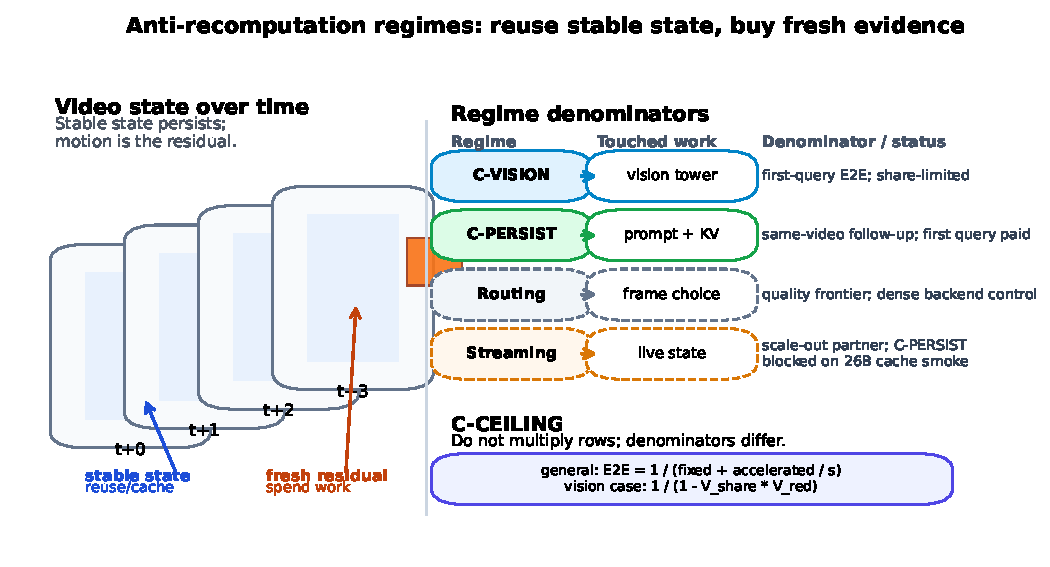
\includegraphics[width=\linewidth]{generated/figures/regime_overview.pdf}
  \caption{Graphical overview. Video has persistent state; the runtime should
  reuse that state where the validation gate allows it and buy fresh evidence
  where the scene, query, or cache topology requires it. C-PERSIST is the
  after-ingest follow-up win; C-CEILING is the denominator guardrail; C-VISION
  is bounded measured first-query skipped work; candidate C-STREAM remains the
  state-update target rather than a fourth headline.}
  \label{fig:regime-overview}
\end{figure}

\section{Introduction}

Video VLMs spend a surprising amount of time rediscovering what they already
know. A benchmark clip is sampled into several frames, many of those frames are
visually redundant, and the stack still pays again for vision encoding,
prefill, or both. The same waste appears in repeated follow-up questions on the
same video, and it becomes even more obvious in live streams where most of the
scene remains stable for long stretches. The interesting question is no longer
whether redundancy exists. It does. The question is where that redundancy can
be removed without breaking the answer.

That sounds like one problem, but it is really three. First-pass inference is
limited by whatever share of wall-clock the vision tower actually owns.
After-ingest follow-up queries on the same video are a different regime: once
the prefix has been paid, prompt reuse can dominate. Benchmark routing under a
fixed dense backend is different again: it tells us whether a training-free
policy preserves quality, not whether the backend has already been rewritten to
skip wall-clock work. Reuse is not one knob. It is three different regimes
with three different ceilings.

We therefore center a broader anti-recomputation story. The fresh-video
headline is Gemma vision-tower pruning: measured end-to-end gains on VideoMME,
MVBench, and TOMATO, with magnitude governed by a simple
share$\times$reduction ceiling. The largest local multipliers come from
persistent-KV reuse on Qwen, where follow-up questions about the same video
drop to sub-second latency. The routing lane then explains the boundary: why
temporal placement of fresh computation matters more than novelty magnitude,
and why semantic-substitution claims must stay separate from sparse-path
speedup claims.

The same thesis also survives contact with deployment-style workloads. In the
deployment-scale streaming evaluation, same-video follow-up latency is 0.8\,s
on Gemma 4 26B, streaming VideoMME reports 13$\times$ ViT reduction and
\mbox{$\sim$50$\times$} dominant-pipeline reduction, selected real-video
regimes report 4.2--4.5$\times$ end-to-end speedups, and an active-scene RTSP
demo still cuts ViT calls by 14.3$\times$ over a 60\,s window. Those numbers
come from a different protocol and stay labeled that way in the paper. They
matter because they show that the benchmark story survives operational
settings.

We make three contributions:
\begin{itemize}[leftmargin=1.5em]
\item We show that training-free mid-layer vision-tower pruning yields measured
first-pass end-to-end gains on frozen Gemma video-VLM runs, and that those
gains are predicted surprisingly well by a simple ceiling law,
$1 / (1 - V_{\mathrm{share}} V_{\mathrm{red}})$.
\item We show that after-ingest follow-up queries are a much larger reuse
opportunity: persistent-KV reuse on Qwen2.5-VL-7B-4bit reduces same-video
follow-up latency to roughly conversational timescales, with 47.2$\times$
speedup at 8 frames and a clean safe envelope through 16 frames.
\item We provide mechanism and boundary evidence for why these gains are
regime-dependent. On clean-tree Qwen holdouts, a bounded-staleness routing
planner preserves the quality--compute frontier, beats novelty-ranked dense
selection, and shows that fresh-compute placement over time matters more than
novelty magnitude alone.
\end{itemize}

\begin{sectiontodo}{Tighten the opening once the final venue and title settle}
The scientific structure is now the right one, but the opening still needs a
last pass for voice and compression after the final venue template lands. Keep
the dry precision; do not let this turn back into either a Qwen-only methods
note or a second streaming paper.

\textcolor{todoBorder}{Source pointers: \path{paper/priority.md},
\path{paper/claim-matrix.md},
\path{paper/publishability-status.md},
\path{paper/framing.md},
\path{codec-through-sam/paper/publishability-status.md}.}
\end{sectiontodo}

\section{Related Work}

The closest systems neighbor is CodecSight \cite{codecsight}, which also tries
to avoid unnecessary visual processing by using compressed-video structure
before the rest of the model consumes the content. The difference is both in
signal and in target. CodecSight uses decoder-native motion vectors and
residuals and is evaluated on streaming anomaly detection; our current local
implementation uses a pixel-domain proxy because that is what our MLX stack can
exercise today, and our main benchmark evaluations target temporal-reasoning QA
on TOMATO \cite{tomato} and MVBench \cite{mvbench}.

Trained codec-native approaches answer a different question. CoPE-VideoLM
\cite{copevideolm}, Deja Vu \cite{dejavu}, and older compressed-video pipelines
such as CoViAR \cite{coviar} learn how motion, residual, or reused
representations should enter the model. That is valuable prior art, but it does
not settle the deployment question we care about here: how much redundancy a
frozen stack can exploit before retraining or representation learning enters
the picture.

Another family reduces visual cost after tokens already exist. FastV
\cite{fastv}, FastVID \cite{fastvid}, FlashVID \cite{flashvid}, VisionZip
\cite{visionzip}, SparseVLM \cite{sparsevlm}, VScan \cite{vscan}, and STTM
\cite{sttm} prune or merge visual tokens using attention-derived, density, or
feature-similarity signals. Those methods are adjacent but not identical to our
setting. Their signal usually lives after visual tokens exist. Our routing lane
asks an earlier question: can we decide where fresh computation should land in
time before the full dense backend pays for every frame again?

Long-horizon reuse and systems co-design are also relevant. QuickVideo
\cite{quickvideo} explicitly co-designs decode and prefill. ReKV \cite{rekv},
VLCache \cite{vlcache}, and StreamingVLM \cite{streamingvlm} study how cached
visual or KV state can be reused across requests or over long contexts. That
line of work is especially relevant to our persistent-KV contribution: the
paper's largest local speedups do not come from a better frame selector, but
from refusing to repay the same prefix when the next question is about the same
video.

SimpleStream \cite{simplestream} is also an important streaming baseline
because it argues that a strong recent-frame window can match or outperform
heavier streaming-memory systems on modern benchmarks. That critique matters
directly for our streaming lane: any cache or memory mechanism has to beat a
strong recency baseline under matched budget, not just beat a strawman.

More conceptually, our framing is adjacent to approximate computing
\cite{rinardapprox}: skipping work under an explicit quality budget. The
difference is that the skipped work here is temporal visual recomputation, and
the guardrail is benchmark fidelity rather than an application-specific numeric
tolerance.

Our position is therefore narrower and more explicit than a generic
``efficient-video-VLM'' claim. We study training-free anti-recomputation for
frozen video VLMs, separating first-pass reuse, after-ingest reuse, and
mechanism-validation routing. The paper is not a claim that pixel differencing
is the final signal. It is a claim that careful temporal reuse is already worth
studying before the full codec-native path lands.

\begin{sectiontodo}{Freeze the final comparison table against the primary papers}
The mechanism families are now in the right buckets, but a submission version
still needs a tighter final comparison table with exact titles, venues, and one
checked headline metric per cited method.

\textcolor{todoBorder}{Source pointers: \path{docs/related-work-table.md},
\path{docs/literature-map-2026-04-16.md},
\path{paper/framing.md}.}
\end{sectiontodo}

\section{Method}

\subsection{Problem Setting}

We study three forms of temporal reuse on frozen video-VLM stacks:

\begin{itemize}[leftmargin=1.5em]
\item \textbf{First-pass visual pruning:} skip or reduce vision-tower work
before the rest of the model pays for it.
\item \textbf{After-ingest follow-up reuse:} keep the expensive prefix from the
first query and ask the next question against the same video.
\item \textbf{Routing under a fixed dense backend:} substitute cached visual
state to test whether answer quality survives, even when the benchmark path has
not yet been rewritten into a sparse wall-clock implementation.
\end{itemize}

These are related, but they are not interchangeable. They are kept
analytically separate because they measure different kinds of reuse.

\subsection{Temporal Planner}

For adjacent frames, the routing path computes a per-block statistic on the RGB
difference plane. The implementation supports mean difference, max-absolute
difference, changed-pixel fraction, and top-$k$ mean over the block. In the
best current clean-tree Qwen policy, the statistic is \texttt{max\_abs}. Fixed
thresholds partition blocks into \emph{static}, \emph{shifted}, and
\emph{novel} regions. These names are historical planner labels, not literal
codec semantics: today they mean low, medium, and high pixel-domain change.

The block geometry is derived from the model's vision configuration rather than
hard-coded. On Qwen2.5-VL, planner decisions line up with the merged-token
spatial grid so cached features can be substituted back into the dense path at
the same geometry the benchmark runner already understands.

\subsection{Bounded Staleness}

Reuse without age control drifts. The planner therefore carries a
bounded-staleness counter: even a block that continues to look reusable must be
refreshed after its age exceeds a configured limit. The clean-tree policy used
in the paper sets that limit to four frame steps. That choice is not cosmetic.
It is the main reason the planner survives TOMATO, where temporally concentrated
evidence punishes policies that keep trusting a stale region simply because the
local pixel difference remains small.

We summarize routing budget by converting block-level reuse into an effective
fresh-frame count,
\[
f_{\mathrm{eff}} = 1 + (N - 1)(1 - r_{\mathrm{reuse}}),
\]
where $r_{\mathrm{reuse}}$ is the mean active-region reuse ratio. This gives
the Qwen routing results a common x-axis with dense-$N$ baselines: how much
fresh visual budget the policy effectively spent.

\subsection{Vision-Tower Pruning and Persistent-KV}

The other two mechanisms operate at different points in the stack.

The Gemma path patches the vision tower after an internal layer, keeps only a
fraction of the tokens, and scatters the result back so downstream geometry is
unchanged. The resulting first-pass speedup is constrained by how much of total
wall-clock the vision tower owns. That is why the paper reports the
scatter-back ceiling
\[
\mathrm{E2E} \le \frac{1}{1 - V_{\mathrm{share}} V_{\mathrm{red}}},
\]
where $V_{\mathrm{share}}$ is the dense vision share and $V_{\mathrm{red}}$ is
the observed reduction in vision time.

The persistent-KV path answers a different question. Here the user has already
paid for the first query on a video. The next question about that same video
reuses the prompt cache and only appends a short textual suffix. The result can
be dramatically faster, but it is explicitly an \emph{after-ingest} claim. It
is not a claim about faster first-pass understanding of fresh videos.

\subsection{What Is Actually Skipped}

The paper keeps semantic substitution and wall-clock skipping separate. The
Qwen routing runner can replay or substitute cached features to test whether the
answer survives. That is enough to study the quality--compute frontier. It is
not enough to claim an end-to-end speedup until the backend itself skips timed
work. The Gemma and persistent-KV lanes do change measured wall-clock and
therefore support speedup claims. The Qwen routing lane does not yet. That
choice is deliberate.

\begin{sectiontodo}{Add the overview figure and final algorithm box}
The prose now matches the paper's current scope, but the final manuscript still
needs a compact visual that makes three distinctions obvious: first-pass
pruning, after-ingest prompt reuse, and Qwen routing as mechanism validation
rather than measured sparse execution.

\textcolor{todoBorder}{Source pointers: \path{src/codec_through/temporal.py},
\path{src/codec_through/novelty_pruning.py},
\path{src/codec_through/pruned_vision_tower.py},
\path{scripts/run_kv_cache_session.py},
\path{paper/claim-matrix.md}.}
\end{sectiontodo}

\section{Experimental Setup}

\subsection{Benchmarks and Workloads}

The paper uses three workload families, because the contribution is not a
single benchmark trick and the protocols are not interchangeable.

The routing mechanism is evaluated on sparse after-ingest QA holdouts: TOMATO
\cite{tomato} and a frozen motion-heavy MVBench slice \cite{mvbench}. These
are the cleanest settings for testing whether training-free temporal reuse
preserves answers at lower effective fresh-frame budgets.

The first-pass speedup story uses Gemma 4-E4B-4bit on Video-MME
\cite{videomme}, MVBench, and TOMATO at 8-frame settings, plus dev-expansion
cells and deeper frame-count probes. The after-ingest persistent-KV story uses
repeated follow-up questions on short Video-MME clips, where the same video is
queried multiple times and prompt reuse is therefore meaningful.

The streaming and UI studies are kept separate from those benchmark claims.
They are native-rate or deployment-style evidence, not replacements for the
main evaluation.
By design, sparse after-ingest QA uses pixel-diff on sampled decoded frames,
while the companion streaming lane uses H.264 metadata at native frame rate.
The signals are protocol-specific, not interchangeable.

\subsection{Models, Hardware, and Preprocessing}

The Qwen routing and persistent-KV experiments use Qwen2.5-VL-7B-Instruct-4bit
through MLX-VLM on Apple Silicon. The dense wall-clock baseline and the
persistent-KV scaling curve use the same local stack on an M3 Air with 16\,GB
unified memory. The first-pass vision-pruning results use Gemma 4-E4B-4bit on
the same general MLX environment. The deployment-scale streaming evaluation
uses a separate RTSP and screen-recording pipeline with Gemma 4 26B.

For benchmark comparability, the main-path runs use uniform global sampling at
8 frames and square-pad plus resize to 560\,$\times$\,560. The routing planner
operates on decoded RGB frames. Padding-aware reuse accounting is reported
separately from raw padded reuse in the artifact summaries; paper-facing
effective-budget numbers use active-region reuse rather than trivially static
padded borders.

\subsection{Metrics and Reporting Discipline}

We report different metrics for different regimes because the paper would be
misleading otherwise.

For Qwen routing, the paper reports accuracy, dense-versus-cached agreement,
parse failures, and effective fresh frames. For Gemma first-pass pruning, it
reports end-to-end speedup, vision-time reduction, accuracy delta, and the
share$\times$reduction ceiling prediction. For persistent-KV, it reports
follow-up latency, speedup relative to the first query, prefix coverage, and
accuracy delta between baseline and session modes.

All automated main-text assets are generated from checked-in artifact summaries.
If a result is advisory, imported, or still provisional, the manuscript says so
explicitly instead of letting the build silently promote it.

\begin{sectiontodo}{Add the final hardware/software table and release sentence}
This section still needs one compact table with model names, hardware, frame
counts, question protocol, and scorer type, plus a final public-release
sentence once the artifact bundle is frozen.

\textcolor{todoBorder}{Source pointers: \path{docs/benchmark-taxonomy.md},
\path{docs/benchmark-setup.md},
\path{docs/methodology/performance.md},
\path{docs/methodology/preprocessing.md},
\path{research/benchmark_manifests/}.}
\end{sectiontodo}

\section{Measured Anti-Recomputation Gains}

The strongest measured results in this paper appear when the reused stage
actually owns meaningful wall-clock. Those gains are not one number. They are
regime-dependent, and the figure below is designed to make that obvious rather
than hide it.

\IfFileExists{generated/tables/headline_results.tex}{
\begin{table}[H]
\centering
\caption{Main speedup cells. Rows use different denominators; C-CEILING explains why they do not multiply.}
\label{tab:headline-results}
\scriptsize
\setlength{\tabcolsep}{2pt}
\renewcommand{\arraystretch}{\PaperTableStretch}
\begin{tabularx}{\linewidth}{@{}>{\raggedright\arraybackslash}p{0.12\linewidth} Y >{\raggedright\arraybackslash}p{0.15\linewidth} >{\raggedright\arraybackslash}p{0.10\linewidth} Y >{\raggedright\arraybackslash}p{0.12\linewidth}@{}}
\toprule
Regime & Setting & Speedup denominator & Gain & Validation / notes & Evidence \\
\midrule
After-ingest repair & Qwen adaptive repair breadth & cold/repaired follow-up & 14.90--35.92$\times$ & choice 0/93; correct 0/93; cold-all-query ratio 15.28--35.97$\times$ & repair breadth \\
After-ingest repair & Qwen fixed \(K=1\) repair breadth & cold/repaired follow-up & 9.48--20.37$\times$ & choice 0/93; correct 0/93; pathological follow-ups 0/62 & repair breadth \\
After-ingest raw & Qwen raw warm reuse, 16f & cold/cached follow-up & 91.1$\times$ & 0.807\,s median; $\Delta$acc +0.000 & aggregate-clean; unrepaired \\
After-ingest raw & Qwen raw warm reuse, 8f & cold/cached follow-up & 47.2$\times$ & 0.815\,s median; $\Delta$acc -0.048 & within criterion \\
First-pass & Gemma VideoMME 8f holdout & first-query E2E & 1.113$\times$ & $\Delta$acc +0.000 & aggregate-clean \\
First-pass & Gemma sparse vision, 32f short & first-query E2E & 1.316$\times$ & choice agreement 100\%; $\Delta$acc +0.000; dense parse 0; sparse parse 0 & \PaperStack{clean}{timed-skip} \\
First-pass & Gemma MVBench 8f holdout & first-query E2E & 1.407$\times$ & $\Delta$acc -0.033; timing-attribution caveat & advisory \\
First-pass & Qwen sparse vision, 16f \(kr_V=0.85\) & first-query E2E & 1.032$\times$ & $\Delta$acc -0.050; vision reduction 13.6\%; parse failures 0; agreement 81.7\% & format gate; low gain \\
\bottomrule
\end{tabularx}
\end{table}

}{
\draftnote{Run \texttt{make paper-sync} to generate the headline results table.}
}

\begin{figure}[H]
  \centering
  \IfFileExists{generated/figures/headline_results.pdf}{
    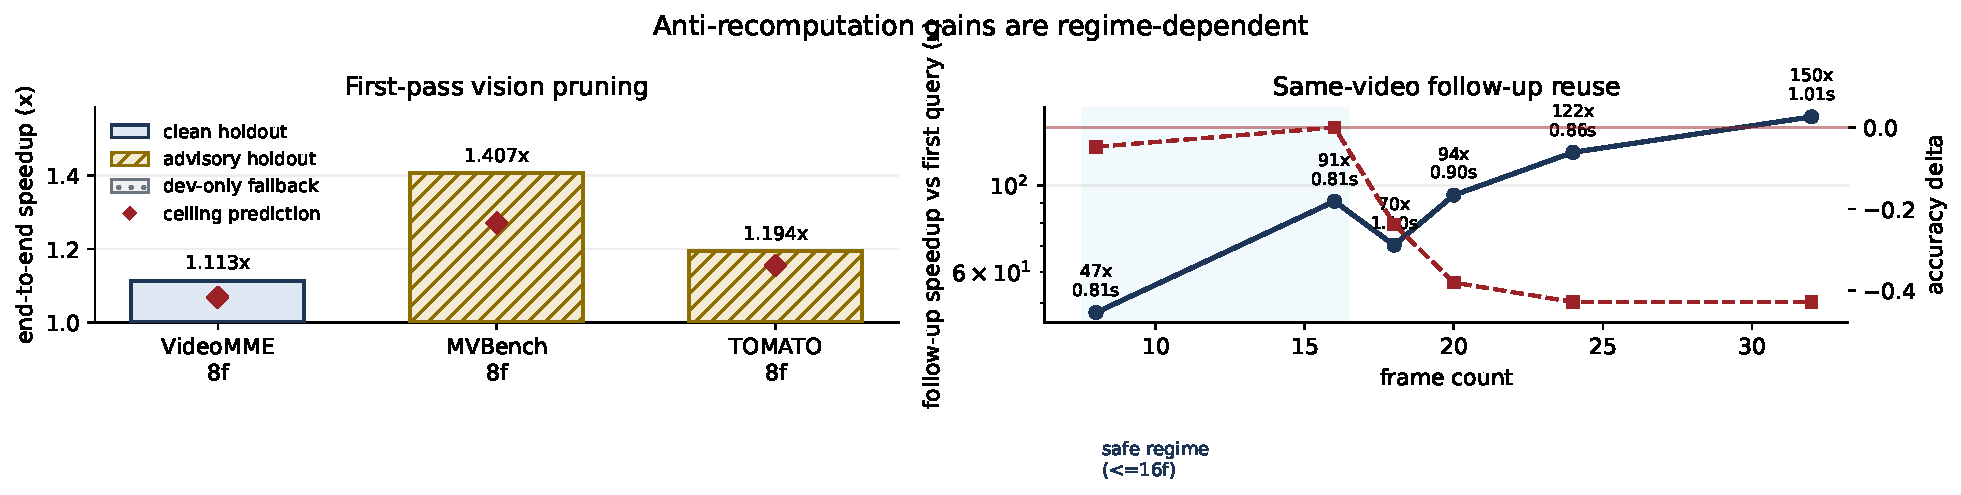
\includegraphics[width=\linewidth]{generated/figures/headline_results}
  }{
    \fbox{\parbox{0.9\linewidth}{Run \texttt{make paper-sync} to generate the headline results figure.}}
  }
  \caption{Headline anti-recomputation results by regime. Left: first-pass
  Gemma vision-pruning speedups with scatter-back ceiling predictions. Right:
  Qwen persistent-KV follow-up speedups versus frame count, with accuracy delta
  tracked separately. Hatched bars indicate advisory or dev-only status rather
  than clean holdout.}
  \label{fig:headline-results}
\end{figure}

\subsection{Orders Of Magnitude For Reuse, Modest Multipliers For Fresh Video}

The largest multipliers here belong to after-ingest reuse: 47.2$\times$ at 8
frames and 91.1$\times$ at 16 frames, both with sub-second follow-up latency.
That is not a contradiction with the smaller first-pass numbers. It is the
expected consequence of reusing an already-paid prefix instead of pruning only
one stage of a fresh-video pass.

\subsection{First-Pass Gains Are Real, But Share-Limited}

Fresh-video first-pass gains are smaller because they are share-limited. Gemma
vision-tower pruning still produces measured end-to-end gains before any
same-video caching trick enters the picture. VideoMME 8f is clean at
1.113$\times$ with zero aggregate accuracy delta. MVBench 8f is stronger still
at 1.407$\times$, with a small accuracy loss and an advisory thermal note
because the short decode window makes the old relative gate too strict for
scheduler-scale jitter. TOMATO 8f is advisory as well: the freshly pulled
upstream rerun reports 1.194$\times$ with a favorable-direction 19\,ms thermal
miss.

Their magnitude tracks the dense share owned by the vision tower. The same
pruning mechanism gives smaller gains on VideoMME than on MVBench because
VideoMME is less vision-dominated at this geometry. That is exactly what the
ceiling law predicts.

\subsection{After-Ingest Reuse Is The Big-Number Regime}

Persistent-KV answers a different question: once the first query on a video has
already paid the full prompt cost, how cheap can the next question become? On
Qwen2.5-VL-7B-4bit, the answer is already large enough to matter. At 8 frames,
follow-up latency drops to 815\,ms median with 47.2$\times$ speedup and
$-0.048$ aggregate accuracy delta. At 16 frames the speedup rises to
91.1$\times$ while the accuracy delta returns to 0. Within the current
$\leq$16f envelope, the result is both fast and empirically clean. Past that
point the curve keeps rising, but the fidelity boundary appears. That is a
useful result in its own right. The big numbers are tied to a concrete
after-ingest regime with a measurable safe envelope.

\subsection{The Story Is Stronger Because The Regimes Are Separate}

The measured first-pass gains and the after-ingest gains complement rather than
compete with each other. First-pass pruning says there is real work to skip on
fresh videos, but the ceiling is share-limited. Persistent-KV says that once a
video has already been ingested, the next question is a much larger reuse
opportunity. The Qwen routing section that follows explains why: temporal
placement of fresh compute decides whether the answer survives.

\begin{sectiontodo}{Lock the final promotion boundary for advisory cells}
The current figure and table are accurate, but the manuscript still needs a
final venue-facing decision on how aggressively to surface advisory rows in the
main text versus the appendix. VideoMME is clean. MVBench and TOMATO are
strong, but they should keep their caveats visible.

\textcolor{todoBorder}{Source pointers: \path{paper/priority.md},
\path{paper/claim-matrix.md},
\path{research/experiments/2026/2026-04-21-phase-1_51V-session3-findings.md},
\path{research/experiments/2026/2026-04-21-phase-1_51V-session4-findings.md},
\path{research/experiments/2026/2026-04-19-phase-1_55A-persistent-kv-findings.md},
\path{research/experiments/2026/artifacts/phase1_55A_*},
\path{codec-through/research/experiments/2026/2026-04-21-phase-1_51V-session5-findings.md}.}
\end{sectiontodo}

\section{Routing Mechanism and Quality--Compute Frontier}

The Qwen routing lane is the cleanest explanation for why training-free
anti-recomputation can work at all. It tells us what kind of temporal signal
is useful, what kind is too blunt, and where the semantic-substitution story
stops.

\subsection{Clean-Tree Holdout Frontier}

On TOMATO motion, the clean base policy matches dense-8 accuracy while spending
only 3.55 effective fresh frames instead of 8.0. On MVBench motion, the same
clean base policy reaches a higher point estimate than dense-6 while spending
less visual refresh: 0.600 accuracy at 4.06 effective fresh frames versus
0.567 at 6.0 fresh frames. At \(n=30\), that is a pointwise Pareto frontier
observation, not a statistical victory lap. Those are not wall-clock claims.
They are benchmarked statements about preserved answer quality at lower
effective visual budget.

\subsection{Automated Snapshot}

\IfFileExists{generated/tables/lane_a_holdout.tex}{
\begin{table}[H]
\centering
\caption{Audited Qwen holdout frontier. The higher-stability MVBench refinement is discussed in text but not plotted.}
\label{tab:lane-a-holdout}
\small
\renewcommand{\arraystretch}{\PaperTableStretch}
\begin{tabular}{lllrrrl}
\toprule
Benchmark & Policy & Relation & Acc. & Fresh & Comparator & Comparator acc. \\
\midrule
TOMATO & planner base & tie & 0.333 & 3.55 & dense-8 (8) & 0.333 \\
MVBench & planner base & frontier & 0.600 & 4.06 & dense-6 (6) & 0.567 \\
\bottomrule
\end{tabular}
\end{table}

}{
\draftnote{Run \texttt{make paper-sync} to generate the automated holdout table.}
}

\begin{figure}[H]
  \centering
  \IfFileExists{generated/figures/lane_a_pareto.pdf}{
    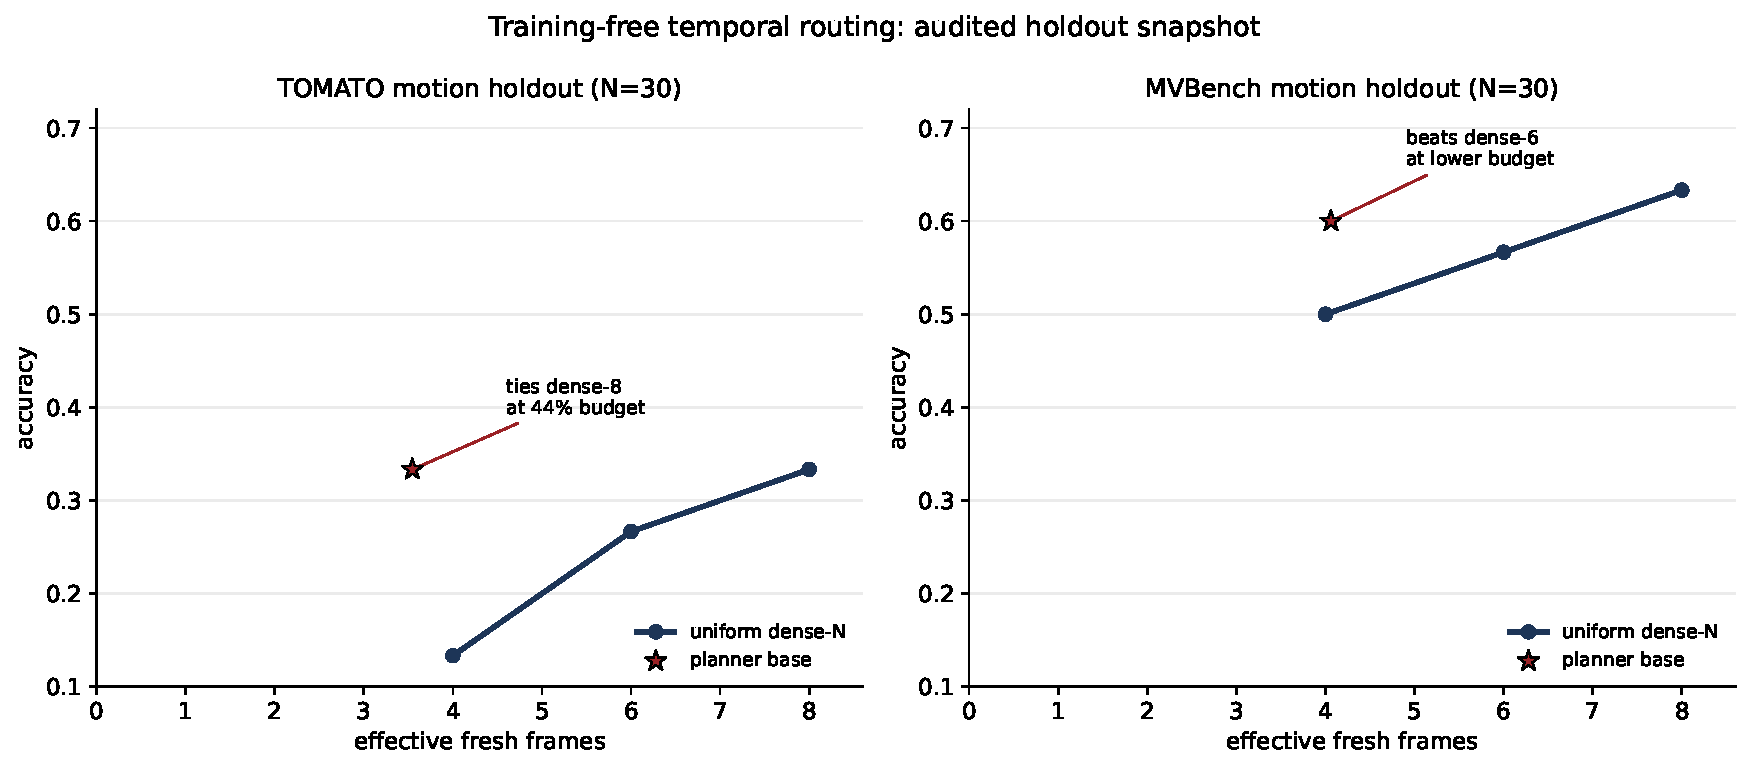
\includegraphics[width=\linewidth]{generated/figures/lane_a_pareto}
  }{
    \fbox{\parbox{0.9\linewidth}{Run \texttt{make paper-sync} to generate the Lane A Pareto figure.}}
  }
  \caption{Clean-tree Qwen holdout frontier from canonical artifact summaries.
  The automated manuscript snapshot intentionally excludes the MVBench
  \texttt{sticky4} variant because the current artifact is dirty-tree and
  remains supplementary until rerun clean.}
  \label{fig:lane-a-pareto}
\end{figure}

The omitted MVBench \texttt{sticky4} refinement remains scientifically
interesting: it reaches 0.633 accuracy at 4.49 effective fresh frames and
therefore matches dense-8 at 56\% of the fresh-frame budget. The current
artifact is still dirty-tree, so the default manuscript snapshot keeps it out
of the main figure on purpose.

\subsection{Novelty Magnitude Alone Is Not Enough}

The most important baseline in this repo is not another cached policy; it is a
non-cached novelty-ranked dense baseline. This baseline asks whether the cached
planner is merely doing smart frame selection in disguise. It is not.

\begin{table}[H]
\centering
\caption{Novelty-ranked dense baseline imported from the phase~1.34 note. This
table is still hand-carried from the authoritative note because a stable
checked-in artifact path for these summaries has not yet been wired into
\texttt{paper-sync}.}
\label{tab:novelty-ranked-dense}
\begin{tabular}{llrr}
\toprule
Benchmark & $N$ & Uniform dense & Novelty-ranked dense \\
\midrule
TOMATO & 4 & 0.133 & 0.133 \\
TOMATO & 6 & 0.267 & 0.167 \\
TOMATO & 8 & 0.333 & 0.233 \\
MVBench & 4 & 0.500 & 0.567 \\
MVBench & 6 & 0.567 & 0.567 \\
MVBench & 8 & 0.633 & 0.567 \\
\bottomrule
\end{tabular}
\end{table}

On TOMATO, novelty ranking hurts once the budget rises above four frames. On
MVBench, it helps at $N=4$ but then saturates and fails to improve with larger
budgets. The cached base policy beats every novelty-ranked dense cell on both
benchmarks. The point is not that novelty is useless. It is that temporal
placement is the real objective, and novelty magnitude alone is a poor proxy
for it.

\subsection{Pixel Statistics Predict Features Only Weakly}

To understand why routing can still work when pixel statistics are crude, we
ran a feature-change oracle that correlates blockwise pixel statistics with
blockwise ViT feature change on cached dense features.

\begin{table}[H]
\centering
\caption{Best point-prediction correlations from the feature-change oracle.}
\label{tab:feature-oracle}
\begin{tabular}{lccc}
\toprule
Benchmark & Best statistic & Pearson $r$ & Spearman $r$ \\
\midrule
TOMATO & mean & 0.233 & 0.177 \\
MVBench & changed-pixel fraction & 0.504 & 0.489 \\
\bottomrule
\end{tabular}
\end{table}

These are weak-to-moderate correlations. That is the point. The best routing
statistic in the planner, \texttt{max\_abs}, is not the best point predictor on
either benchmark. Routing and point prediction are different objectives: the
planner only needs a signal that spends scarce refresh budget in the right part
of the clip often enough to preserve the answer.

\begin{sectiontodo}{Finish the mechanism appendix boundary}
The routing section is now in the right role, but three things still need
cleanup before submission: wire the novelty-ranked dense table to stable
artifacts, either rerun or appendix-ize \texttt{sticky4}, and tighten the
caption language after the final venue template lands.

\textcolor{todoBorder}{Source pointers: \path{paper/claim-matrix.md},
\path{research/experiments/2026/2026-04-15-phase-1_20-tomato-motion-slice-enlargement.md},
\path{research/experiments/2026/2026-04-15-phase-1_21-mvbench-motion-slice-enlargement.md},
\path{research/experiments/2026/2026-04-17-phase-1_34-novelty-ranked-dense.md},
\path{research/experiments/2026/2026-04-17-phase-1_36-feature-change-oracle.md}.}
\end{sectiontodo}

\section{Scale-Out Streaming and Deployment Evidence}

The largest reported operational gains appear when the model keeps revisiting
nearly the same visual state. We treat the Gemma 4 26B streaming stack as a
scale-out lane for the same anti-recomputation questions, not as decorative
application color. The current draft still labels those rows separately because
they use a different model, machine, runtime, and streaming protocol; promoting
them to first-class evidence requires the same artifact-compatible outputs and
matched baselines used by the local experiments. Under the current protocol,
the stack reports 0.8\,s median same-video follow-up latency at 10--18$\times$
speedup, paired Streaming VideoMME results with 13$\times$ fewer ViT calls and
\mbox{$\sim$50$\times$} less dominant measured subpipeline compute, and selected
real-video regimes with 4.2--4.5$\times$ end-to-end speedups. ``Dominant
measured subpipeline'' is the instrumented high-cost streaming segment in that
runtime, not a full end-to-end denominator. Reported live-camera measurements
show the same regime dependence in the wild: one post-fix RTSP demo reduces
ViT calls by 14.3$\times$ over an active 60\,s window, while broader
scene-dependent 5--300$\times$ live-counter ranges remain appendix-weighted
until matched baselines land.

These rows are not local headline cells yet. They are included because they
show the scale of the operational regime where a stable scene is queried
repeatedly. The right current claim is that the scale-out lane exercises the
same anti-recomputation structure under a native streaming workload, not that
its counters can be multiplied into the local C-VISION or C-PERSIST numbers.
The paper-facing goal is to turn this lane into a first-class
\emph{streaming state reuse} evaluation with the same paired outputs, cache
correctness smoke tests, low-FPS / screenshot-polling / recency baselines, and
artifact bundle as the controlled local runs.

Smaller-$N$ UI studies stay strictly illustrative, not headline-bearing. The
sectional-scroll case studies remain explicitly weaker than the paired
streaming and real-video measurements above, and the contact-sheet imagery
below is qualitative rather than quantitative. The main-body evidence for this
section is the deployment table below.

\begin{table}[H]
\centering
\caption{Heterogeneous operational evidence for the streaming/deployment
regime. Metric type is shown explicitly because these rows mix component
counters, end-to-end timing, and live observations with different sample sizes
and denominators. Smaller UI and demo case studies are discussed in text and
kept clearly weaker than the paired streaming rows below. All scale-out rows are
pending artifact harmonization before they become first-class evidence in the
same claim graph as the local runs.}
\label{tab:real-apps}
\footnotesize
\renewcommand{\arraystretch}{1.16}
\begin{tabularx}{\linewidth}{@{}
  >{\raggedright\arraybackslash}p{0.18\linewidth}
  >{\raggedright\arraybackslash}p{0.16\linewidth}
  >{\raggedright\arraybackslash}X
  >{\raggedright\arraybackslash}p{0.16\linewidth}
@{}}
\toprule
Setting & Metric type & Outcome & Evidence class \\
\midrule
Streaming VideoMME (Gemma 26B) & component counter + accuracy & reported paired N=60: 13$\times$ fewer ViT calls; $\sim$50$\times$ less dominant measured subpipeline compute in the instrumented streaming segment; 58.3/60.0/61.7\% (stream/token-prune/dense), all within the reported $\pm$12 pp 95\% CI & scale-out stream benchmark \\
Real-video paired regimes (Gemma 26B) & end-to-end timing & reported 4.2--4.5$\times$ end-to-end speedup on talking-head and surveillance-style real-video measurements & scale-out real-video benchmark \\
Gemma 26B same-video follow-up & follow-up latency & reported N=20 VideoMME follow-up subset: 0.8\,s median follow-up; 10--18$\times$ faster than cold prefill; aggregate accuracy 65.0\% with and without KV reuse & scale-out follow-up benchmark \\
Live-camera pipeline & live component counter & reported single-system counter: 14.3$\times$ fewer ViT calls on one active 60\,s RTSP window (701 decoded frames / 49 ViT calls); broader 5--300$\times$ scene-dependent range remains appendix-weighted live-counter evidence & scale-out live measurement \\
\bottomrule
\end{tabularx}
\end{table}

The Qwen composition experiments do not yet reproduce this operational story as
a fidelity-preserving stack. The original stacked run reproduced the speedup
side but failed the accuracy budget. The dense-first-query admission successor
restores first-query aggregate correctness and leaves a follow-up-only
near-miss, but it also shows why the claim boundary must stay strict. The
long-bucket continuations now measure follow-up image-token activity directly
and find none: all follow-up image tokens are cache-served under the current
prompt-cache path, and every tested long-Q0 keep rate misses the target
fidelity/speed band.
That lane is therefore dense-first-query admission plus K-cache reuse rather
than proof of active follow-up vision pruning. That is why
Table~\ref{tab:real-apps} is operational evidence rather than part of the local
C-VISION or C-PERSIST headline rows.

\begin{figure}[H]
  \centering
  \IfFileExists{generated/figures/streaming_snapshot_contact_sheet.png}{
    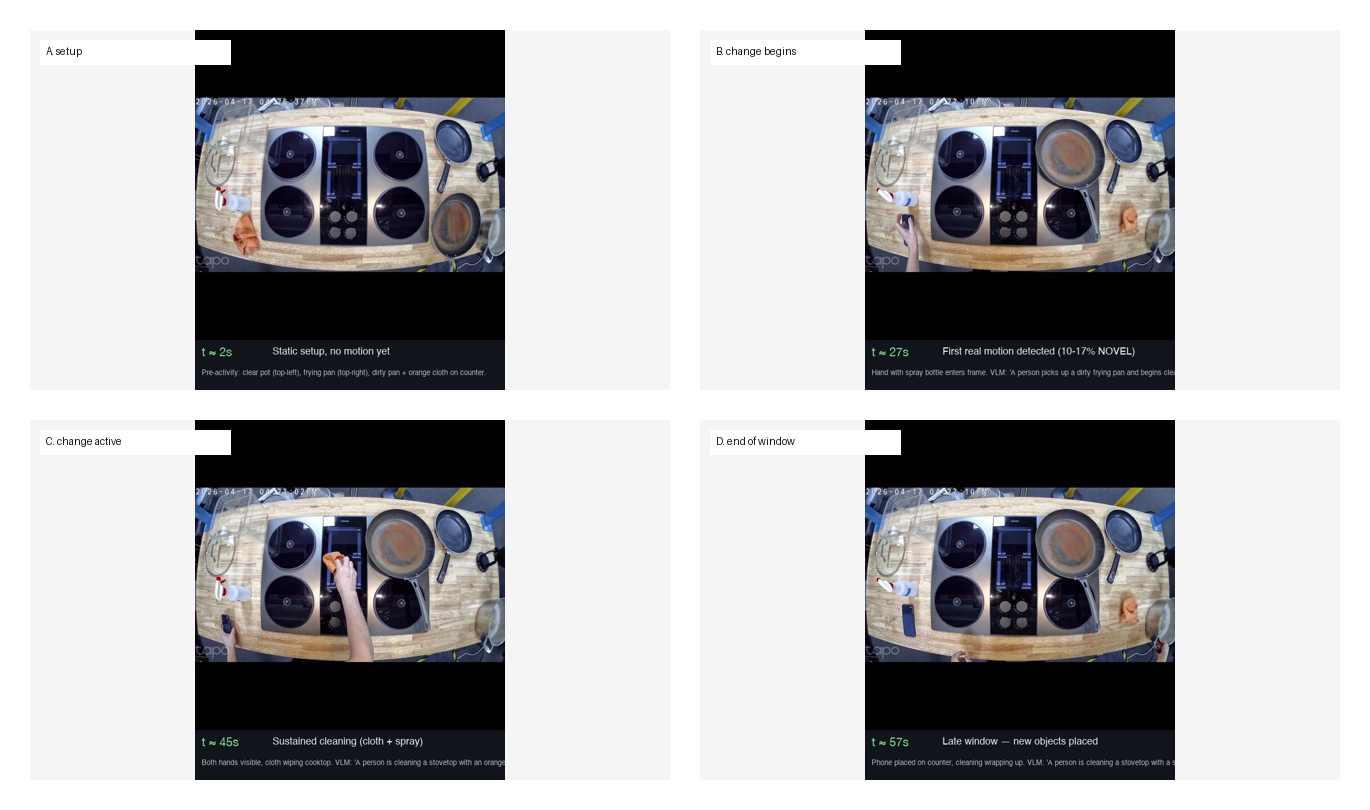
\includegraphics[width=\linewidth]{generated/figures/streaming_snapshot_contact_sheet.png}
  }{
    \fbox{\parbox{0.9\linewidth}{Run \texttt{make paper-sync} to generate the streaming/UI contact sheet or a placeholder.}}
  }
  \caption{Representative imagery from the post-fix RTSP demo. These snapshots
  are qualitative only; they illustrate an active-scene live deployment, but
  the quantitative deployment claims in Table~\ref{tab:real-apps} come from the
  paired streaming, real-video, and live-camera measurements rather than from
  this contact sheet.}
  \label{fig:streaming-contact-sheet}
\end{figure}

The current streaming evidence does not yet close a full systems-reviewer
checklist. The paper still lacks the screenshot-polling baseline, low-FPS dense
baseline, SimpleStream-style recency baseline, broader UI diversity, and a
dedicated stale-cache failure case. The scale-out lane should next run the same
claim axes as the local paper: a cache-correctness smoke test, C-PERSIST
same-video follow-up replication, measured sparse-ViT / ceiling validation,
native streaming matched baselines, and a raw re-export of the large sparse
exactness artifact with item IDs, paired outputs, parse failures, and
confidence intervals. What it already suggests is that the same
anti-recomputation principle can appear outside sparse benchmark slices, in the
regime where users keep asking the same system about nearly the same scene.

\begin{sectiontodo}{Keep scale-out evidence reviewer-safe}
The next useful additions are a screenshot-polling baseline, a wider UI set,
and one concrete failure case where stale-cache decisions break trust. Keep the
section tied to the scale-out evidence above. Smaller UI claims such as
sectional scroll, threshold tuning, or affine-axis mechanism variants should
stay appendix-weighted until their evidence is cleaned up further.

\textcolor{todoBorder}{Remaining work: add cache-correctness smoke artifacts
for the 26B stack, a C-PERSIST scale-out replication, measured sparse-ViT /
ceiling validation, screenshot-polling and low-FPS dense baselines, broader UI
coverage, and one stale-cache failure case before making the streaming lane
carry more of the headline.}
\end{sectiontodo}

\section{Discussion: Toward VLM-Native Media}

The experiments above are intentionally conservative: frozen models, explicit
evidence classes, no speed claim where the backend did not skip timed work.
That conservatism should not hide the bigger implication. Existing media
pipelines already contain cheap temporal structure, but most video VLM stacks
consume the final RGB frames as if every frame were equally new. Anti-
recomputation asks a systems question before it asks for a new model: what did
the media pipeline already know, and why did the VLM pay to rediscover it?

\subsection{Unchanged Is Only The First Case}

Same-position reuse is the simplest regime: if a patch did not change, reuse
its visual evidence. But video codecs also exploit a richer fact: many things
change predictably. Objects translate, cameras pan, forward-driving cameras
produce structured expansion, and occlusions create localized new evidence.
The current paper earns evidence mostly for static-to-medium-motion benchmark
regimes and for same-video follow-up reuse. It does \emph{not} yet prove
motion-compensated feature reuse, driving-specific routing, or sensor-fusion
caching. Those directions follow naturally from the failures and ceilings we
measured, so they belong in the paper's agenda rather than in the headline
claim.

\begin{table}[H]
\centering
\caption{Application regimes as evidence targets, not generic motivation. The
right policy depends on the redundancy structure and on what failure would
cost.}
\label{tab:application-regimes}
\footnotesize
\renewcommand{\arraystretch}{1.22}
\begin{tabularx}{\linewidth}{@{}
  >{\raggedright\arraybackslash}p{0.18\linewidth}
  >{\raggedright\arraybackslash}p{0.22\linewidth}
  >{\raggedright\arraybackslash}p{0.26\linewidth}
  >{\raggedright\arraybackslash}X
@{}}
\toprule
Regime & Redundancy structure & Candidate routing policy & Evidence status / risk \\
\midrule
Static cameras, factories, surveillance, stove/countertop & stable background,
localized entrants, rare decisive events & persistent visual memory plus
bounded-staleness refresh around moving regions & closest to current evidence;
needs stronger application baselines and event-window recall \\
\addlinespace[0.25em]
Screen and UI video & exact-copy regions, glyph changes, scrolling, cursor
motion & screen-content path with exact-copy, OCR/glyph, and high-frequency
guards & planned specialization; current VideoMME audit under-samples scroll/pan \\
\addlinespace[0.25em]
Forward driving & structured ego-motion, border entry, independently moving
objects & pose/flow-conditioned refresh with protected object and boundary
regions & future lane; should not be inferred from same-position reuse \\
\addlinespace[0.25em]
Egocentric, FPV, drones & jerky motion, parallax, frequent occlusion & global
stabilization or multi-reference cache before reuse & current benchmark mix is
the wrong corpus for this claim \\
\addlinespace[0.25em]
Robotics / VLA & static workspace plus gripper/object/contact zones and hard
deadlines & protected ROIs, p95/p99 latency budgets, guarded dense fallback & future
systems lane; answer-stability QA is not a control-safety metric \\
\addlinespace[0.25em]
Games and HUD-heavy streams & stable HUD, structured camera regimes, repeated
interaction states & HUD anchors plus event-triggered world refresh & future
application lane; likely high reuse but unmeasured here \\
\bottomrule
\end{tabularx}
\end{table}

\paragraph{Robotics is a different contract.}
Robotics is not just another row in an application table. It changes the
optimization target from average answer stability to deadline-safe perception.
A plausible safety contract is protected reuse, not maximal reuse: test
policies that always refresh the gripper, manipulated object, contact boundary,
goal receptacle, newly entering regions, and any sensor-disagreement zone;
reuse aggressively elsewhere; and report p95/p99 latency, deadline misses,
fallback rate, and task success instead of only QA accuracy. We do not claim
that evidence here. We name it because it is the natural systems lane once
anti-recomputation leaves offline QA.

\subsection{From Video Streams To State Streams}

The scale-out streaming rows are the concrete predecessor of this interface:
they are not yet a standardized C-STREAM result, but they show why a
perception-rate state stream is the right deployment abstraction to test.

The same logic extends beyond RGB video. A robot, vehicle, or factory cell may
carry multiple cameras, depth or ToF, IMU/odometry, event sensors, object
tracks, calibration, timestamps, and confidence estimates. These side channels
are not semantic-saliency oracles. They are cheaper refresh and uncertainty
oracles: RGB says what a region looks like; depth says whether geometry moved;
IMU says whether apparent motion is explained by the camera; event sensors
flag onset; multi-camera geometry distinguishes occlusion from disappearance.
The VLM-native interface we want is therefore not ``more frames,'' but a
synchronized state-update stream that tells the runtime where fresh visual
evidence is worth buying.

\subsection{Codec Signals Are Requirements Probes}

Classical codecs are hand-engineered prediction systems: predict a reference,
send motion and residual surprise, transform and quantize under a rate-
distortion objective, and make the result cheap enough for hardware. That
objective was designed mainly for human viewing. Standards work is already
moving toward machine consumption, including MPEG-AI Part 2 Video Coding for
Machines \cite{mpegvcm}, JPEG AI \cite{jpegai}, and event-data coding efforts
such as JPEG XE \cite{jpegxe}. Older object/layer media ideas, including
MPEG-4 Visual object coding \cite{mpeg4visual}, also show that rectangular RGB
frames were not the only conceivable abstraction. The analogy to object-based
audio such as Dolby Atmos \cite{dolbyatmos} is useful but only as an analogy:
the goal is not theatrical rendering, but a synchronized stream of
model-facing state updates.

Our role in that trajectory is narrower. We are not designing the future codec
here. We use VLM behavior to motivate candidate requirements for that future
interface:

\begin{table}[H]
\centering
\caption{How current limitations motivate future media-interface requirements.
These are hypotheses and candidate design requirements, not current
measured claims.}
\label{tab:media-requirements}
\small
\renewcommand{\arraystretch}{1.14}
\begin{tabularx}{\linewidth}{@{}
  >{\raggedright\arraybackslash}p{0.40\linewidth}
  >{\raggedright\arraybackslash}X
@{}}
\toprule
Observed limitation or boundary & Future VLM-native media should expose \\
\midrule
Mean block difference misses small but decisive events & residual
concentration, changed-pixel fraction, onset flags, and max-age state \\
Novelty-ranked dense frames can cluster budget in the wrong place & temporal
coverage constraints, event-window hints, and placement-aware scheduling \\
Same-position reuse weakens under camera motion & camera pose, global motion,
depth-aware flow, and boundary-entry flags \\
Predictably moving objects are not static but are not arbitrary either &
object IDs, masks, tracks, motion uncertainty, and multi-reference state \\
Human-compression artifacts can hide model-critical text or color & task-aware
text, chroma, palette, and high-frequency metadata \\
Sparse regions may be awkward for today's tensor kernels & tensor-friendly
active tiles, projector-consistent groups, and regular batched sparse layouts \\
RGB alone confuses lighting, geometry, and contact & synchronized depth/ToF,
event, IMU/odometry, timestamp, and confidence sidecars \\
\bottomrule
\end{tabularx}
\end{table}

\paragraph{Layered world-state media.}
One useful mental model is a machine-facing analogue of object/layer media:
static background memory, camera pose, object tracks and masks, motion
uncertainty, residual surprise, text/glyph events, event-camera onset,
depth/ToF changes, timestamps, and confidence. The model would render or
refresh dense visual evidence only where the state update requires it. This is
not a current codec implementation; it is the interface pressure revealed by a
paper about paying for the wall again.

\paragraph{Beyond zero-change inference.}
The current result is useful precisely because it is frozen-model and
training-free. It identifies where an existing model already tolerates reuse
and where it does not. The model-changing version should train around those
traces rather than ignore them: learned recache gates, codec-conditioned token
types, P-frame or delta encoders, and cache-state-aware attention can all use
the failure cases and routing logs produced by this paper as supervision.
There is also a training-compute hypothesis: if future VLMs learn from
state-update streams rather than dense RGB frame stacks, they may spend the
same training FLOPs on more temporal coverage, more queries per clip, or harder
event windows. We do not measure that here. The caveat is important:
post-vision-tower feature caching does not directly become an end-to-end training
speedup when the vision encoder is trainable, because cached features
approximate or break the gradient path. The training version likely needs
model-native delta encoders, differentiable refresh gates, or teacher/student
traces rather than dropping inference caches into pretraining unchanged.

\paragraph{Beyond video.}
The general pattern is not unique to pixels. Any expensive encoder over a
slowly changing state stream can, in principle, benefit from a cheap freshness
oracle: financial order books, industrial telemetry, scientific sensor arrays,
long medical monitoring streams, or logs from embodied agents. Video is the
right starting point because temporal redundancy is explicit, codecs already
extract motion and residual signals, and the cost of visual encoding is large
enough to matter. Other domains need their own state variables and failure
contracts; the transferable lesson is anti-recomputation under a measured
quality--compute frontier, not pixel differencing itself. The transfer rule is
strict: the domain needs slowly changing state, an oracle cheaper than the
encoder, expensive recomputation, and task-specific paired-failure metrics.
Without all four, anti-recomputation is just a metaphor.

\subsection{Open Experiments}

Several high-value brainstorm items remain deliberately outside the current
evidence boundary.

The near-term research questions are reader-facing, not bookkeeping. Does
semantic substitution become a real wall-clock win when the backend actually
skips measured vision work? Does temporal placement of fresh compute beat
novelty magnitude under matched budgets? Can saved compute buy broader
temporal coverage rather than only lower latency? Can answer-margin and
paired-drift features predict when reuse will fail? Which application baselines
make deployment claims credible rather than anecdotal? How far does paired
stability extend when a user asks dialogue-like follow-up questions about the
same video, and what repair schedule prevents drift from accumulating?

The longer-range agenda is the VLM-native media ladder: object/state delta
sidecars; sensor-fusion world-state streams with depth/ToF, event, pose, and
timestamp layers; compute-denial robustness; learned recache gates;
codec-conditioned token types; learned delta encoders; and hardware-aware
active-tile decode. These ideas follow from the measurements above, but they
remain future work unless they receive their own reproduced artifacts.

The same anti-recomputation principle may also rotate into generative video
and audio. A video generator or world model could reuse latent hidden state
across denoising steps or autoregressive chunks when predicted motion and
residual uncertainty are low, then refresh around occlusion, entropy spikes, or
new-object events. Audio has a similar shape but a different trap: quiet is not
the same as irrelevant, so onset, phoneme boundaries, speaker changes, and
prosody matter more than energy alone. These are domain rotations, not evidence
claims in this paper.

The long-term version is simple to state: video for machines should become a
timeline of state updates, not only dense RGB frames. Static background,
camera motion, dynamic objects, text, events, depth, sensor confidence, and
time can all be first-class evidence. This paper is the first rung: a careful
training-free measurement of where anti-recomputation works today, where it
fails, and what future media systems should stop making the model rediscover.

\section{Limitations and Reproducibility}

The paper makes three kinds of claim, and each one breaks differently. That is
the main limitation to manage.

For first-pass Gemma pruning, the evidence is now good enough for a main
results section, but not every cell is equally clean. VideoMME is clean.
MVBench and TOMATO are advisory because the measured gains survive, but the
thermal caveats are still visible and should remain visible in the text.
Architecture breadth is also still limited: the first-pass measured speedup
story is Gemma-first today.

For persistent-KV, the numbers are much larger, but the regime is narrower.
These are \emph{after-ingest} claims: the first query on the video still pays
full freight, and the gain only appears when subsequent questions concern that
same video. The safe envelope is also finite. Through 16 frames the local curve
is clean. Beyond that, fidelity degrades quickly.

For Qwen routing, the opposite caveat applies. The holdout evidence is clean
and useful, but it is still a quality--compute frontier result under a fixed
dense backend. It should not be inflated into a measured sparse-execution
speedup claim until the backend actually skips timed work.

The streaming lane is the smallest-$N$ evidence class in the paper. It is
there because it shows the practical regime where redundancy becomes large, not
because it already closes the full systems-reviewer checklist. The paper still
needs a screenshot-polling baseline, broader UI coverage, and a cleaner local
codec-native bridge if that lane is going to carry more of the headline later.

The paper is nevertheless being built to be reproducible. Automated main-text
figures and tables are generated from checked-in artifact summaries, the
appendix records the repo commits used for the sync, and imported or advisory
evidence is labeled as such instead of being silently promoted into the
headline figures. The paper builds locally with the checked-in
\texttt{make paper-*} targets plus `tectonic` or a fuller TeX stack.

\begin{sectiontodo}{Freeze the public artifact and release language}
Before submission, this section still needs the final public-release sentence,
artifact-bundle wording, and one last pass on which advisory results stay in
main text versus move to the appendix.

\textcolor{todoBorder}{Source pointers: \path{paper/priority.md},
\path{paper/claim-matrix.md},
\path{docs/reproduction-status.md},
\path{docs/methodology/performance.md},
\path{docs/clip-policy.md}.}
\end{sectiontodo}

\section{Conclusion}

The paper began with a small absurdity: much of the video did not change, and
the model paid anyway. The measured answer is not one multiplier.
Same-video follow-up reuse is the big-number regime: after the first query
pays, selective re-prefill and repaired-cache inheritance give
14.90--35.92$\times$ follow-up speedup with no observed paired drift across
the 93-query breadth setting. Fresh-video pruning is smaller but real, and its
gains obey the stage-share ceiling. Streaming is the natural deployment target,
but the evaluated 26B-class bundle shows why topology-safe cache reuse and strong
low-FPS baselines are gates, not details.

The boundaries are the science. Aggregate accuracy can hide answer drift.
Semantic substitution is not timed skipped work. Component wins do not multiply
just because the table numbers look good next to each other.

The larger direction is simple: VLMs should not have to rediscover repeated
frames back into state. Future media streams for machines should expose change,
motion, uncertainty, objects, text, sensor time, and active tiles directly.
Anti-recomputation is one empirical step from video-as-frames toward
video-as-world-state updates.

\begin{sectiontodo}{Final bibliography polish still needed}
The draft now cites the papers it discusses, but the bibliography is still
maintained manually so the manuscript can build cleanly with the lightweight
local toolchain. Before submission, convert this into the final venue-approved
bibliography workflow and re-check every title, venue string, and author list
against the primary source.

\textcolor{todoBorder}{Source pointers: \path{docs/related-work-table.md},
\path{docs/literature-map-2026-04-16.md},
\path{docs/benchmark-taxonomy.md}.}
\end{sectiontodo}

\begin{thebibliography}{99}

\bibitem{codecsight}
\emph{CodecSight}. arXiv:2604.06036, 2026.

\bibitem{copevideolm}
\emph{CoPE-VideoLM}. arXiv:2602.13191, 2026.

\bibitem{coviar}
\emph{CoViAR: A Codebook-Free Representation for Compressed Video Action Recognition}. arXiv:1712.00636, 2017.

\bibitem{cacheblend}
Jiayi Yao, Hanchen Li, Yuhan Liu, Siddhant Ray, Yihua Cheng, Qizheng Zhang,
Kuntai Du, Shan Lu, and Junchen Jiang.
\emph{CacheBlend: Fast Large Language Model Serving for RAG with Cached
Knowledge Fusion}. EuroSys 2025; arXiv:2405.16444.

\bibitem{dejavu}
\emph{D\'ej\`a Vu}. arXiv:2506.14107, 2025.

\bibitem{eventful}
Matthew Dutson, Yin Li, and Mohit Gupta.
\emph{Eventful Transformers: Leveraging Temporal Redundancy in Vision
Transformers}. ICCV 2023; arXiv:2308.13494.

\bibitem{evoprune}
Yuhao Chen, Bin Shan, Xin Ye, and Cheng Chen.
\emph{EvoPrune: Early-Stage Visual Token Pruning for Efficient MLLMs}.
arXiv:2603.03681, 2026.

\bibitem{fastv}
\emph{FastV: A Fast Compression Framework for Visual Tokens in Vision-Language Models}. arXiv:2403.06764, 2024.

\bibitem{fastvid}
\emph{FastVID: Dynamic Density Pruning for Fast Video Large Language Models}. arXiv:2503.11187, 2025.

\bibitem{fastvlm}
Pavan Kumar Anasosalu Vasu, Fartash Faghri, Chun-Liang Li, Cem Koc, Nate
True, Albert Antony, Gokul Santhanam, James Gabriel, Peter Grasch, Oncel
Tuzel, and Hadi Pouransari.
\emph{FastVLM: Efficient Vision Encoding for Vision Language Models}. CVPR
2025; arXiv:2412.13303.

\bibitem{flashvid}
\emph{FlashVID: Efficient Video Large Language Models via Training-free Tree-based Spatiotemporal Token Merging}. OpenReview ICLR 2026, 2026.

\bibitem{framefusion}
\emph{FrameFusion}. arXiv:2501.01986, 2025.

\bibitem{mvbench}
\emph{MVBench: A Comprehensive Multi-modal Video Understanding Benchmark}. arXiv:2311.17005, 2023.

\bibitem{mpegvcm}
MPEG. \emph{Video Coding for Machines}. \url{https://www.mpeg.org/standards/MPEG-AI/2/}

\bibitem{jpegai}
JPEG. \emph{JPEG AI}. \url{https://jpeg.org/jpegai/}

\bibitem{jpegxe}
JPEG. \emph{JPEG XE activity status}. \url{https://jpeg.org/items/20241121_jpeg_xe_activity_status.html}

\bibitem{hermes}
Haowei Zhang, Shudong Yang, Jinlan Fu, See-Kiong Ng, and Xipeng Qiu.
\emph{HERMES: KV Cache as Hierarchical Memory for Efficient Streaming Video
Understanding}. arXiv:2601.14724, 2026.

\bibitem{llavaprumerge}
Yuzhang Shang, Mu Cai, Bingxin Xu, Yong Jae Lee, and Yan Yan.
\emph{LLaVA-PruMerge: Adaptive Token Reduction for Efficient Large Multimodal
Models}. ICCV 2025; arXiv:2403.15388.

\bibitem{dolbyatmos}
Library of Congress. \emph{Dolby Atmos Master File}. \url{https://www.loc.gov/preservation/digital/formats/fdd/fdd000646.shtml}

\bibitem{mpeg4visual}
Library of Congress. \emph{MPEG-4, Visual Coding, Main Profile}. \url{https://www.loc.gov/preservation/digital/formats/fdd/fdd000048.shtml}

\bibitem{quickvideo}
\emph{QuickVideo: Real-Time Long Video Understanding with System Algorithm Co-Design}. OpenReview TMLR, 2026.

\bibitem{rekv}
\emph{Streaming Video Question-Answering with In-context Video KV-Cache Retrieval}. OpenReview ICLR 2025, 2025.

\bibitem{rinardapprox}
Martin C. Rinard. \emph{Approximate Computing}. CSAIL research overview, 2026. \url{https://people.csail.mit.edu/rinard/research/ApproximateComputing/}

\bibitem{sglang}
Lianmin Zheng, Liangsheng Yin, Zhiqiang Xie, Chuyue Sun, Jeff Huang, Cody Hao
Yu, Shiyi Cao, Christos Kozyrakis, Ion Stoica, Joseph E. Gonzalez, Clark
Barrett, and Ying Sheng.
\emph{SGLang: Efficient Execution of Structured Language Model Programs}.
NeurIPS 2024; arXiv:2312.07104.

\bibitem{sparsevlm}
\emph{SparseVLM: Visual Token Sparsification for Efficient Vision-Language Model Inference}. arXiv:2410.04417, 2024.

\bibitem{sparsevila}
Samir Khaki, Junxian Guo, Jiaming Tang, Shang Yang, Yukang Chen, Konstantinos
N. Plataniotis, Yao Lu, Song Han, and Zhijian Liu.
\emph{SparseVILA: Decoupling Visual Sparsity for Efficient VLM Inference}.
ICCV 2025; arXiv:2510.17777.

\bibitem{simplestream}
\emph{A Simple Baseline for Streaming Video Understanding}. arXiv:2604.02317, 2026.

\bibitem{sttm}
\emph{Multi-Granular Spatio-Temporal Token Merging for Training-Free Acceleration of Video LLMs}. arXiv:2507.07990, 2025.

\bibitem{streamingllm}
Guangxuan Xiao, Yuandong Tian, Beidi Chen, Song Han, and Mike Lewis.
\emph{Efficient Streaming Language Models with Attention Sinks}. ICLR 2024;
arXiv:2309.17453.

\bibitem{streamingvlm}
\emph{StreamingVLM: Real-Time Understanding for Infinite Video Streams}. arXiv:2510.09608, 2025.

\bibitem{tomato}
\emph{TOMATO: Lifting the Impossible in Video Reasoning}. arXiv:2410.23266, 2024.

\bibitem{tome}
Daniel Bolya, Cheng-Yang Fu, Xiaoliang Dai, Peizhao Zhang, Christoph
Feichtenhofer, and Judy Hoffman.
\emph{Token Merging: Your ViT But Faster}. ICLR 2023; arXiv:2210.09461.

\bibitem{videomme}
\emph{Video-MME: The First-Ever Comprehensive Evaluation Benchmark of Multi-modal LLMs in Video Analysis}. arXiv:2405.21075, 2024.

\bibitem{visionzip}
\emph{VisionZip}. arXiv:2412.04467, 2024.

\bibitem{vlcache}
\emph{VLCache: Cache-Efficient Vision-Language Model Serving via Cross-Request Reuse}. arXiv:2512.12977, 2025.

\bibitem{vllm}
Woosuk Kwon, Zhuohan Li, Siyuan Zhuang, Ying Sheng, Lianmin Zheng, Cody Hao
Yu, Joseph E. Gonzalez, Hao Zhang, and Ion Stoica.
\emph{Efficient Memory Management for Large Language Model Serving with
PagedAttention}. SOSP 2023; arXiv:2309.06180.

\bibitem{vscan}
\emph{VScan}. arXiv:2505.22654, 2025.

\end{thebibliography}


\appendix
\section{Source Traceability and Provenance}

The manuscript uses four evidence classes and labels them differently in the
text. \emph{Reproduced-here evidence} comes from \texttt{codec-through-2} and
backs the automated headline assets, the persistent-KV curve, and the Qwen
routing section. \emph{Tracked-upstream evidence} comes from the sibling
\texttt{codec-through} tree when the local manuscript is intentionally tracking
a fresher rerun that has not yet been copied back here. \emph{Scale-out partner
evidence} comes from the separate 26B streaming tree and is restricted to the
streaming and real-application section until artifact harmonization lands.
\emph{Hypotheses or moving results} may be discussed for context, but they are
not allowed into the default automated manuscript snapshot.

This appendix is where that distinction becomes audit-friendly. The repo
provenance table below records the commit pins observed by the manuscript sync
step. Because this draft commits generated paper assets, the primary row can
point to the pre-commit working-tree snapshot that produced the PDF; a
\texttt{-dirty} suffix means the PDF is a working-tree draft, not a
submission-frozen artifact bundle. The final release should regenerate this
table from a clean tag. Within the main text, numbers are written so they can
be traced back to one phase note and one artifact family. When a result is
excluded or downgraded on provenance grounds, the paper says so explicitly. The
best current examples are the MVBench \texttt{sticky4} refinement, Gemma's
matched-parse-failure sparse-vision sweep, and Qwen's conservative low-gain
sparse-vision boundary: all are scientifically useful, but none should be
silently promoted beyond the finite evidence class it actually earned.

\begin{table}[H]
\centering
\caption{Claim/protocol/evidence manifest for the main quantitative assets.}
\label{tab:claim-protocol-manifest}
\tiny
\setlength{\tabcolsep}{1.5pt}
\renewcommand{\arraystretch}{1.06}
\begin{tabularx}{0.99\linewidth}{@{}
  >{\raggedright\arraybackslash}p{0.12\linewidth}
  >{\raggedright\arraybackslash}X
  >{\raggedright\arraybackslash}p{0.14\linewidth}
  >{\raggedright\arraybackslash}p{0.25\linewidth}
@{}}
\toprule
Asset & Claim / protocol & Evidence class & Source / hardware \\
\midrule
Headline table & regime headline cells; first-pass vision-pruning holdout, measured sparse-vision envelope, and after-ingest follow-up & local + tracked-upstream & Phases 1.51V, 1.55A/D/E/F/G/H/I/K, 1.63E/G/H; adaptive mechanism and stage-timing artifacts; Gemma/Qwen local stacks, MLX / M3 Air 16 GB \\
C-CEILING figure & C-CEILING / C-VISION scatter-back validation; first-pass holdout, n=60 stacked-regime audit, matched cross-arch probe, and measured sparse-vision boundary & local + tracked-upstream + local boundary & ceiling data JSON; local Gemma and local Qwen stacks plus tracked-upstream TOMATO rerun; 1.63E/G/H raw artifacts checked in \\
Measured sparse-vision tables & real timed vision-tower work skipped under Gemma and Qwen & local bounded systems evidence & Phase 1.63G Gemma 8/16/32f scaling and Phase 1.63H Qwen 16f keep-rate sweep; Qwen 1.63E 8f boundary \\
C-PERSIST figure & C-PERSIST tested envelope; after-ingest same-video follow-up & local & Phase 1.55A artifacts; Qwen 7B/3B-4bit, MLX / M3 Air 16 GB \\
C-PERSIST repair & 20f/32f same-video selective re-prefill & local bounded recovery & Phases 1.55D/E/F/G/H/I plus adaptive mechanism and stage-timing artifacts; Qwen 7B-4bit, VideoMME short/medium/long + 32f short \\
C-PERSIST sampler sweep & adaptive short-cell practical temperature robustness & local reviewer-defense evidence & Phase 1.55K artifacts; Qwen 7B-4bit, VideoMME short slice, \(T\in\{0.0,0.5,0.7,1.0,1.5\}\) \\
Routing frontier & sparse routing under dense backend & local & Phase 1.20/21/34/36 notes; Qwen 7B-4bit, MLX \\
Gemma routing boundary & second-architecture semantic substitution & local boundary & Phase 1.42 artifacts; Gemma 4-E4B-4bit, TOMATO/MVBench motion holdouts \\
Qwen stacked boundary & session/streaming composition plus cache-boundary attribution & local negative / boundary & Phase 1.30 root-cause + W/X/Y/Z/AB/AC/AD/AF artifacts; Qwen 7B-4bit, VideoMME dev+holdout \\
Paired drift table & paired choice/correctness drift summary & local analysis & Phase 1.61 drift summary built from landed 1.30, 1.42, and 1.55A artifacts \\
Logit-margin scout & dense answer-margin signal is insufficient as a high-precision drift guard & local negative / future guard feature & Phase 1.65 artifacts; 228 scored Qwen paired rows \\
Memory envelope & process working-set characterization across landed families & local reproducibility evidence & Phase 1.66 memory characterization; 78 cells across follow-up reuse, admission/composition, and measured sparse vision \\
Method / limitations & codec-native planner bridge; semantic planner substitution & local semantic evidence & Phase 1.29B artifacts; Qwen 7B-4bit, VideoMME dev/short slices; offline extraction, not latency \\
Scale-out streaming & native-rate streaming paired N=60 & scale-out partner, pending artifact harmonization & deployment report \S2.13.2 / status docs; Gemma 4 26B / M5 Max \\
Scale-out real video & paired real-video regimes & scale-out partner, pending artifact harmonization & deployment report \S2.8 real-video timings; Gemma 4 26B / M5 Max \\
Candidate C-STREAM probes & MV/residual staleness, sectional cache shift, static-camera inflection triggers, and E3 wall-clock instrumentation & scale-out partner mechanism probes, pending harmonized raw artifacts & companion deployment repository decision-log rows 2.02, 2.03-SCROLL, 2.06, 2.06-NEG; E3 findings; Gemma 4 26B / M5 Max \\
Scale-out follow-up diagnostic & Gemma 26B PromptCacheState cross-turn smoke & blocked cache-semantics diagnostic & cross-turn cache-correctness findings; deterministic and within-turn checks pass, cross-turn warm follow-up matches dense on 2/5 \\
Scale-out live & native-rate live camera & scale-out partner, pending artifact harmonization & deployment report \S2.13.1 / live-demo docs; Gemma 4 26B / M5 Max \\
\bottomrule
\end{tabularx}
\end{table}

\begin{sectiontodo}{Freeze this provisional manifest into a submission artifact map}
Before submission, this appendix should expand the provisional manifest above
into a frozen claim-to-artifact map for every table and figure in the paper,
including final hardware strings, exact artifact bundle paths, and any rows
that still move between main text and appendix.

\textcolor{todoBorder}{Source pointers: \path{paper/claim-matrix.md},
\path{docs/reproduction-status.md},
\path{paper/publishability-status.md},
\path{paper/arxiv/generated/tables/repo_provenance.tex}.}
\end{sectiontodo}

\IfFileExists{generated/tables/repo_provenance.tex}{
\begin{table}[H]
\centering
\caption{Repo provenance for the current manuscript sync.}
\label{tab:repo-provenance}
\begin{tabular}{lll}
\toprule
Repo & Commit & Commit date \\
\midrule
codec-through-2 & 1b7c05a40b28 & 2026-04-25 \\
codec-through & 1b7c05a40b28 & 2026-04-25 \\
codec-through-sam & 47acc8d55efe & 2026-04-23 \\
\bottomrule
\end{tabular}
\end{table}

}{
\draftnote{Run \texttt{make paper-sync} to generate the repo provenance table.}
}

\section{Automated Assets and Figure Sources}

Several tables and figures are generated from checked evidence artifacts:
routing frontiers, headline anti-recomputation assets, measured sparse-vision
tables, C-PERSIST repair and stress tables, setup-economics tables, the
random-keep sanity baseline, the scale-out bundle status table, memory
characterization, paired-drift summaries, and source provenance.

The point is scientific rather than procedural: quantitative paper assets
should come from checked rows, not free-form notes or screenshots.

\section{Manuscript Completion Checklist}

\begin{sectiontodo}{Use this appendix as the pre-submission checklist}
Before submission, this checklist should be rewritten as a final appendix item
or deleted. It currently exists to keep the paper honest while the science is
still moving.
\begin{itemize}[leftmargin=1.5em]
\item Freeze the target venue template and stop building on the temporary draft style.
\item Replace every visible TODO box in the main text with final prose or move it to an internal checklist.
\item Rerun or drop every supplementary result that still fails the paper-grade provenance bar, especially MVBench \texttt{sticky4}.
\item Regenerate manual tables from canonical artifacts where stable artifact paths now exist.
\item Keep clean, advisory, tracked-upstream, scale-out partner, and dev-only evidence visibly distinct in the final manuscript.
\item Finalize the public code, artifact, and data-release wording.
\item Build the final arXiv source bundle from a clean tree and verify that no local-only metadata leaks into it.
\end{itemize}
\end{sectiontodo}



\end{document}
